\section{Smooth surfaces in $\mathbb R^3$}

\subsection{Definitions and equivalent characterisations}
Recall that if $V \subset \mathbb R^n$ and $V' \subset \mathbb R^m$, then $f \colon V \to V'$ is smooth if it is infinitely differentiable.

\begin{definition}[Smooth Function on $\mathbb{R}^n$]
	If $Z$ is an arbitrary subset of $\mathbb R^n$, we say that $f \colon Z \to \mathbb R^m$ is \vocab{smooth} at $p \in Z$ if $\exists$ an open ball $p \in B \subset \mathbb R^n$ and a smooth map $F \colon B \to \mathbb R^m$ which extends $f$ such that they agree on $B \cap Z$\footnote{$F\mid_{B \cap Z} = f\mid_{B \cap Z}$}.
	In other words, $f$ is locally the restriction of a smooth map defined on an open set.
\end{definition}

\begin{remark}
	This is useful as it may be difficult to take partial derivatives on $Z$, as when you consider a small deviation from a point $p$ that deviation might not lie in $Z$.
\end{remark} 

\begin{figure}[h] 
    \centering 
    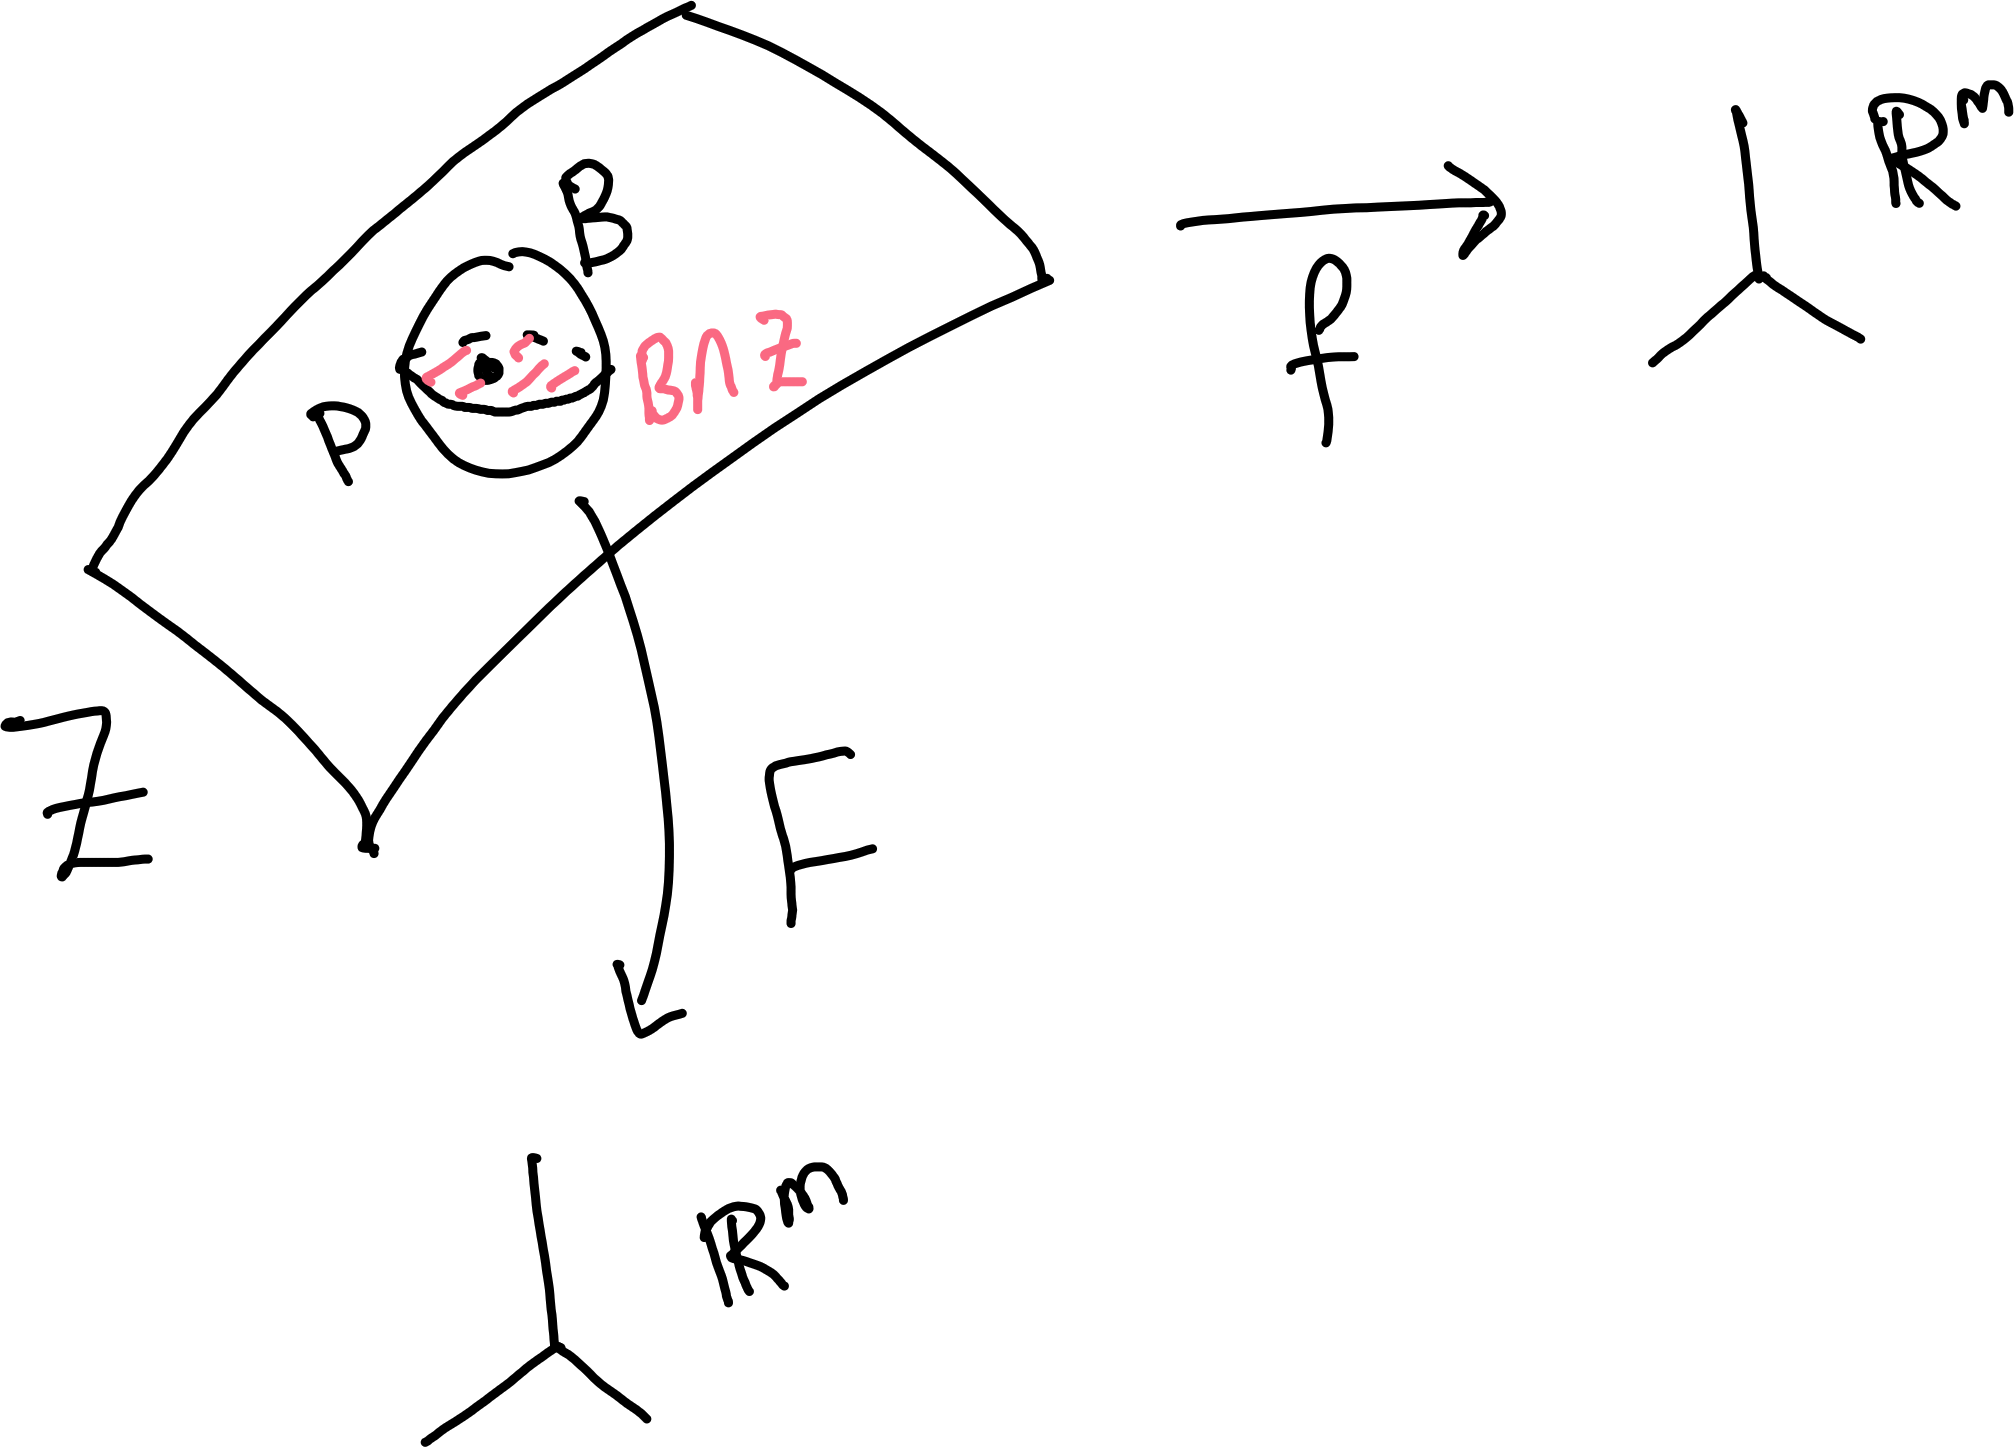
\includegraphics[height=5cm]{03-smooth} 
\end{figure}

\begin{definition}[Diffeormorpishms in $\mathbb{R}^n, \mathbb{R}^m$]
	Let $X \subset \mathbb R^n$ and $Y \subset \mathbb R^m$.
	We say that $X$ and $Y$ are \vocab{diffeomorphic} if $\exists \; f \colon X \to Y$ smooth with smooth inverse.
\end{definition}

\begin{definition}[Smooth Surface in $\mathbb{R}^3$]
	A \vocab{smooth surface in $\mathbb R^3$} is a subset of $\Sigma \subset \mathbb R^3$ s.t. $\forall \; p \in \Sigma$, $\exists$ an open subset $p \in U \subset \Sigma$ that is diffeomorphic to an open set in $\mathbb R^2$.
\end{definition}

In other words, for all $p \in \Sigma$, there exists an open ball $p \in B \subset \mathbb R^3$ such that if $U = B \cap \Sigma$ and there exists a map $F \colon B \to V \subset \mathbb R^2$ smooth s.t. $\eval{F}_U \colon U \to V$ is a homeomorphism, and the inverse map $V \to U \subset \Sigma \subset \mathbb R^3$ is smooth.

So we have two notions of smoothness, one abstract and one based on the ambient space and we need to reconcile them.

\begin{definition}[Allowable Parameterisation]
	Let $\sigma \colon V \to U$ where $V \subset \mathbb R^2$ is open and $U \subset \Sigma \subset \mathbb R^3$ is open in $\Sigma$, such that $\sigma$ is a smooth homeomorphism and $\eval{D\sigma}_x$ has rank 2 for all $x \in V$.
	Then $\sigma$ is called an \vocab{allowable parametrisation}.
	If $\sigma(0) = p$, we say that $\sigma$ is an allowable parametrisation \textit{near} $p$.
\end{definition}

\begin{theorem} \label{thm:1.7}
	For a subset $\Sigma \subset \mathbb R^3$, the following are equivalent (TFAE).
	\begin{enumerate}
		\item $\Sigma$ is a smooth surface in $\mathbb R^3$;
		\item $\Sigma$ is locally the graph of a smooth function, over one of the three coordinate planes: for all $p \in \Sigma$ there exists an open ball $p \in B \subset \mathbb R^3$ and an open set $V \subset \mathbb R^2$ such that
		      \begin{align*}
			      \Sigma \cap B = \qty{(x, y, g(x,y)) \colon g \colon V \to \mathbb R \text{ smooth}}
		      \end{align*}
		      or one of the other coordinate planes;
		\item $\Sigma$ is locally cut out by a smooth function with non-zero derivative: for all $p \in \Sigma$ there exists an open ball $p \in B \subset \mathbb R^3$ and a smooth function $f \colon B \to \mathbb R$ such that
		      \begin{align*}
			      \Sigma \cap B = f^{-1}(0);\quad \eval{Df}_x \neq 0 \ \forall \; x \in B.
		      \end{align*}
		\item $\Sigma$ is locally the image of an allowable parametrisation near all points.
	\end{enumerate}
\end{theorem}

\begin{remark}
	Part (2) implies that if $\Sigma$ is a smooth surface in $\mathbb R^3$, each $p \in \Sigma$ belongs to a chart $(U, \varphi)$ where $\varphi$ is (the restriction of) one of the three coordinate plane projections $\pi_{xy}, \pi_{yz}, \pi_{xz}$ from $\mathbb R^3$ to $\mathbb R^2$.
	Consider the transition map between two such charts.
	{\par
	\centering 
    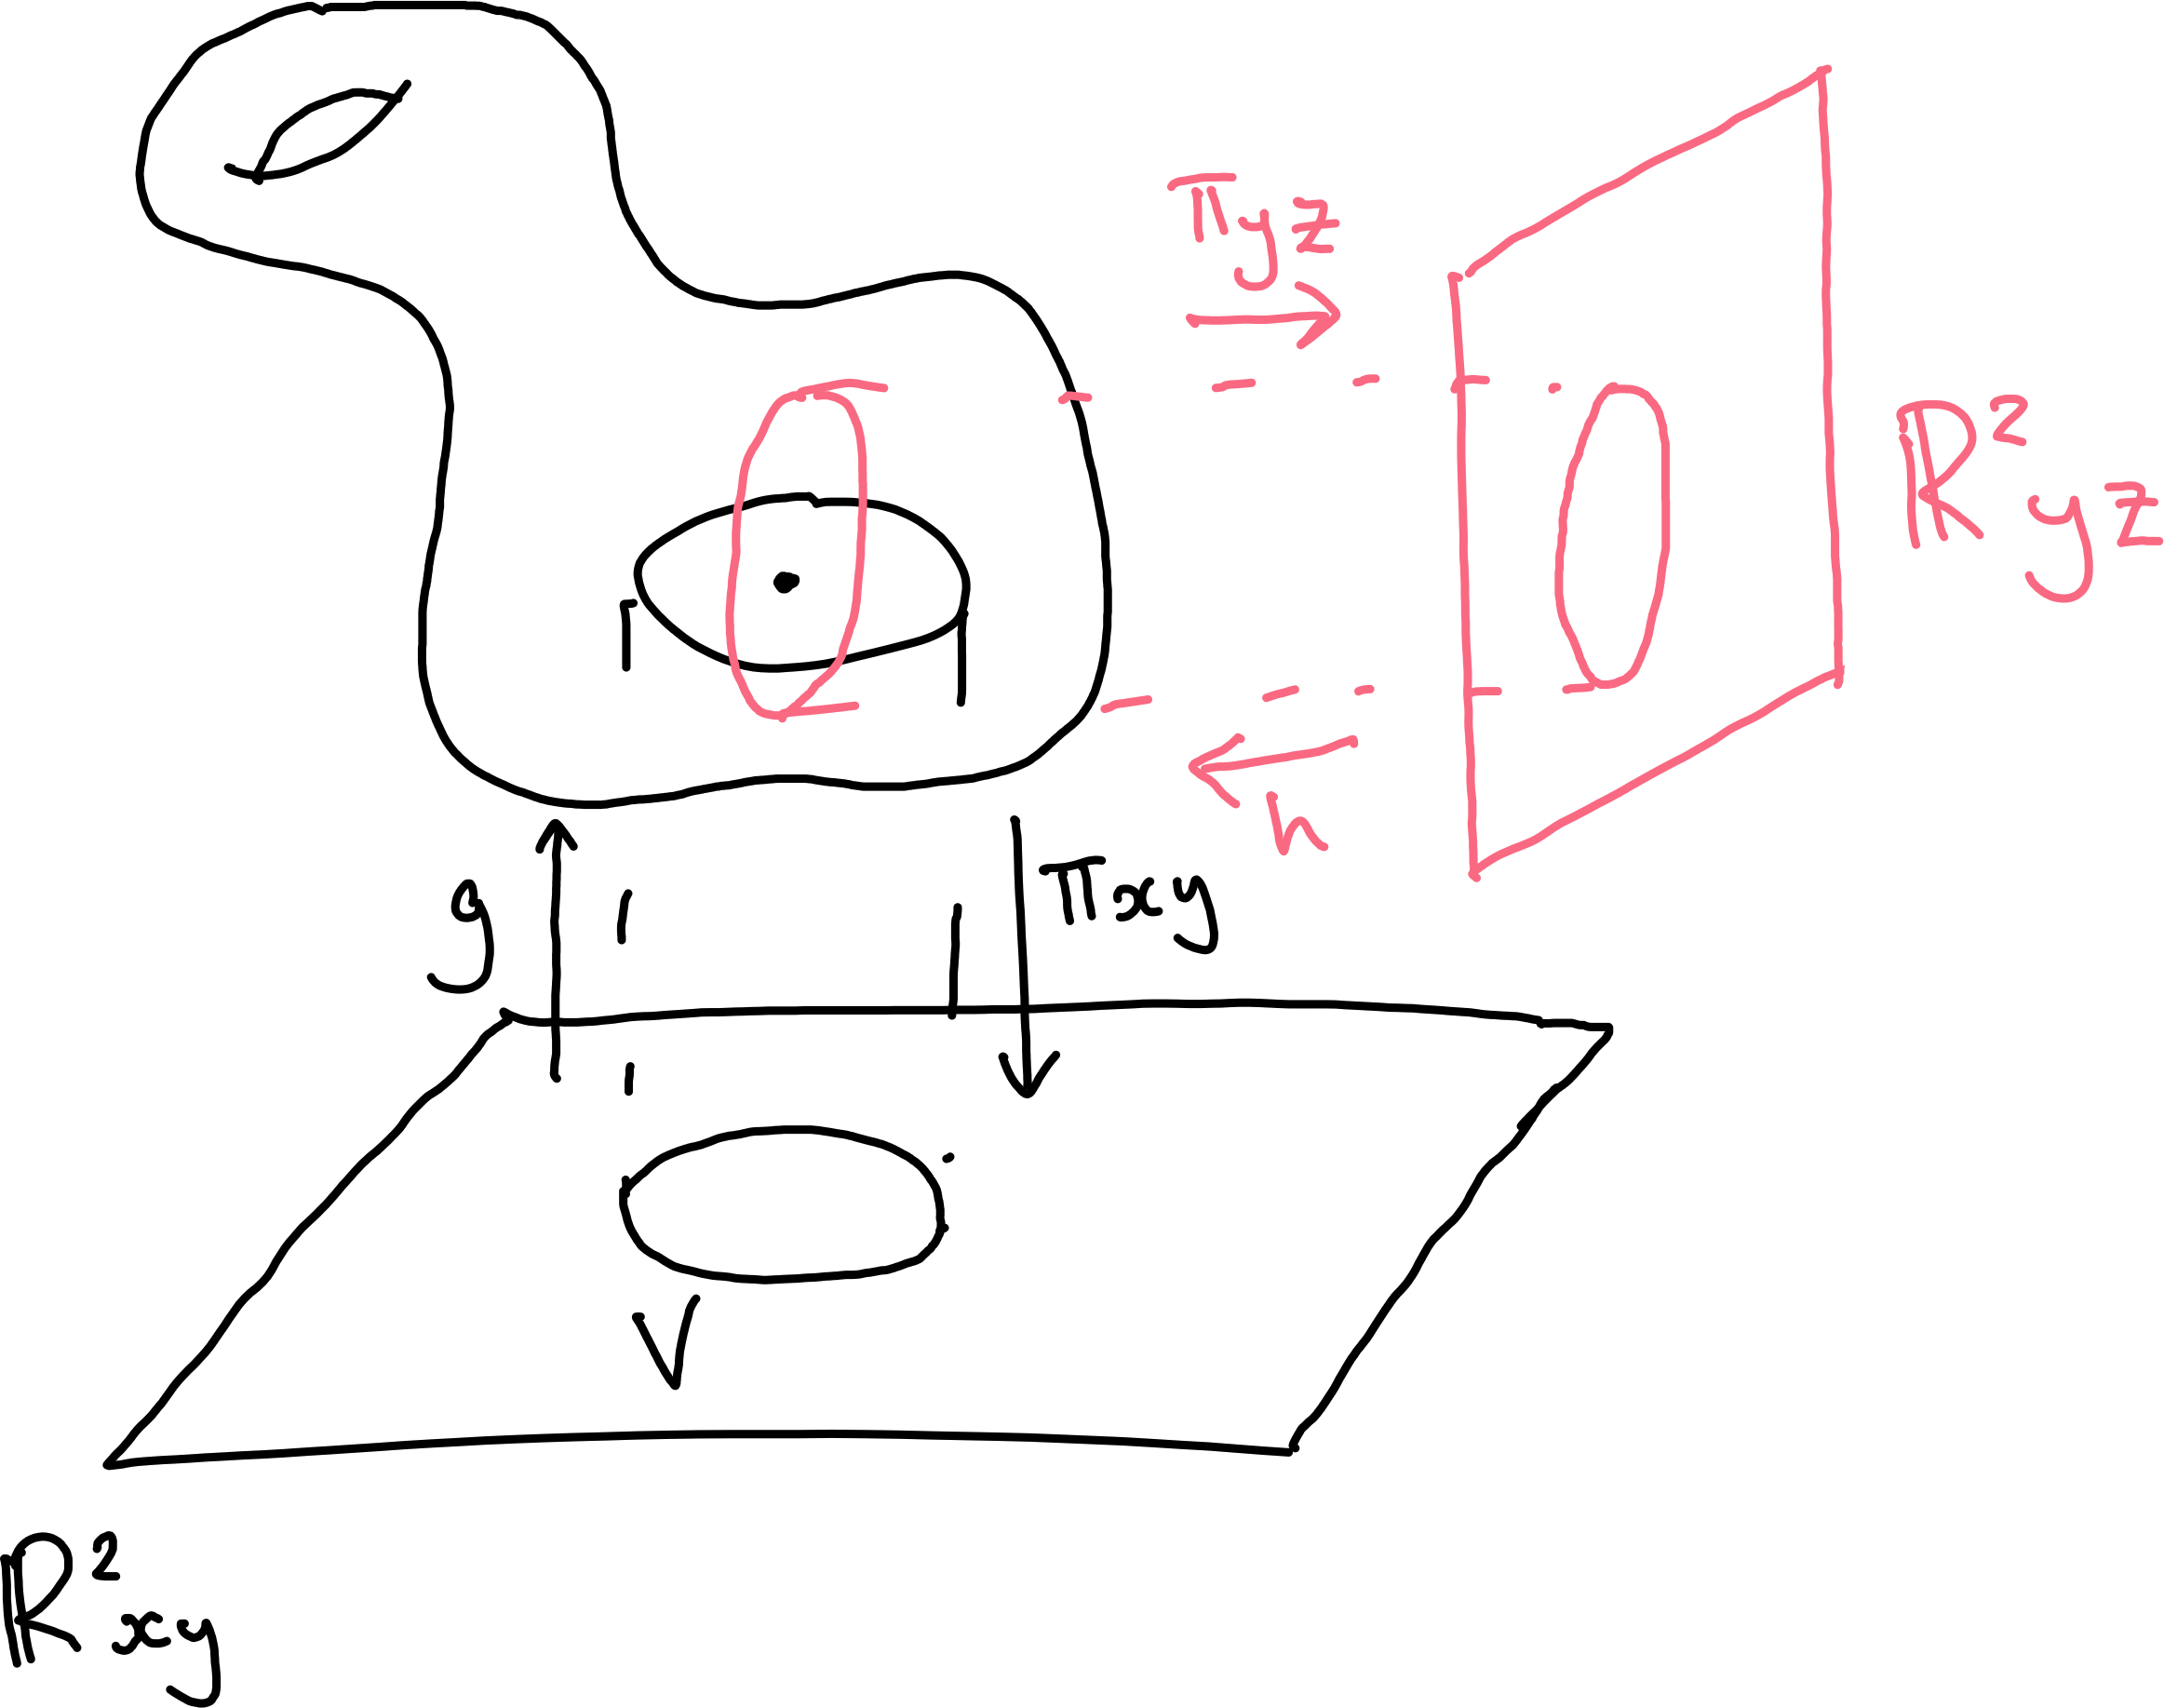
\includegraphics[height=5cm]{03-transitionmapremarks} 
	\par}
	If the two charts are based on the same projection such as $\pi_{xy}$, then the transition map is the identity.
	If they are based on different projections $\pi_{xy}$ and $\pi_{yz}$, then the transition map is
	\begin{align*}
		(x,y) \mapsto (x,y,g(x,y)) \mapsto (y,g(x,y))
	\end{align*}
	which has inverse
	\begin{align*}
		(y,z) \mapsto (h(y,z),y,z) \mapsto (h(y,z),y)
	\end{align*}
	Hence all of the transition maps between such charts are smooth.
	This gives $\Sigma$ the structure of an abstract smooth surface.
\end{remark}
Some of the relations given in the above theorem are easy to prove, but others come as a result of the inverse function theorem.

\subsection{Inverse and implicit function theorems}
\begin{theorem}[Inverse Function Theorem]
	Let $U \subset \mathbb R^n$ be open, and $f \colon U \to \mathbb R^n$ be continuously differentiable.
	Let $p \in U$ and $f(p) = q$.
	Suppose $\eval{Df}_p$ is invertible. \\
	Then there is an open neighbourhood $V$ of $q$ and a differentiable map $g \colon V \to \mathbb R^n$ and $g(q) = p$ with image an open neighbourhood $U' \subset U$ of $p$ such that $f \circ g = \id_V$ and $g \circ f = \id_{U'}$.
	If $f$ is smooth, then $g$ is also.
\end{theorem}

\begin{remark}
	The chain rule then implies that $\eval{Dg}_q = \qty(\eval{Df}_p)^{-1}$.

	The inverse function theorem concerns functions $\mathbb R^n \to \mathbb R^n$, where $\eval{Df}_p$ is an isomorphism.
	If we have a map $\mathbb R^n \to \mathbb R^m$ for $n > m$, then we can discuss the behaviour when $\eval{Df}_p$ is surjective.
	The derivative $\eval{Df}_p$ is an $m \times n$ matrix, so if it has full rank, up to the permutation of coordinates we have that the last $m$ columns are linearly independent.
\end{remark}

\begin{theorem}[Implicit Function Theorem]
	Let $p = (x_0, y_0)$ be a point in an open set $U \subset \mathbb R^k \times \mathbb R^\ell$.
	Let $f \colon U \to \mathbb R^\ell$ be a continuously differentiable map s.t. $p \mapsto 0$ and $\qty(\pdv{f_i}{y_j})_{\ell \times \ell}$ is an isomorphism at $p$. \\
	Then there is an open neighbourhood $V$ of $x_0$ in $\mathbb R^k$ and a continuously differentiable map $g \colon V \to \mathbb R^\ell$ with $x_0 \mapsto y_0$ such that if $(x,y) \in U \cap (V \times \mathbb R^\ell)$, then $f(x,y)=0 \iff y=g(x)$.
	If $f$ is smooth, so is $g$.
\end{theorem}

\begin{proof}
	Let $F \colon U \to \mathbb R^k \times \mathbb R^\ell$ be defined by $(x,y) \mapsto (x,f(x,y))$.
	Then note that
	\begin{align*}
		DF = \begin{pmatrix}
			I & \ast           \\
			0 & \pdv{f_i}{y_j}
		\end{pmatrix}
	\end{align*}
	hence $DF$ is an isomorphism at $(x_0, y_0)$.
	By the Inverse function theorem, $F$ is locally invertible near $F(x_0,y_0) = (x_0,f(x_0,y_0)) = (x_0, 0)$. \\
	Consider an open neighbourhood $(x_0, 0) \in V \times V' \subset \mathbb R^k \times \mathbb R^\ell$, where $V, V'$ open, on which this continuously differentiable inverse $G \colon V \times V' \to U' \subset U \subset \mathbb R^k \times \mathbb R^\ell$ exists, such that $F \circ G = \id_{V \times V'}$. \\
	Then,
	\begin{align*}
		G(x,y) = (\varphi(x,y), \psi(x,y)) \implies F \circ G(x,y) = (\varphi(x,y), f(\varphi(x,y), \psi(x,y))) = (x,y)
	\end{align*}
	Hence $\varphi(x,y) = x$.
	We have $f(x,\psi(x,y)) = y$ when $(x,y) \in V \times V'$.
	This gives $f(x,y) = 0 \iff y = \psi(x,0)$\footnote{Here $y$ is in $V'$ so it is in the image of $f$, i.e. it is $f(a, b)$ for some $a, b$. So $y = 0$ gives us $f(a, b) = 0$. We see that $f(a, \psi(a, 0)) = 0$ so $b = \psi(a, 0)$ defines our surface in $U$}. \\
	We then define $g \colon V \to \mathbb R^\ell$ by $x \mapsto \psi(x,0)$.
\end{proof}

\begin{example}
	Let $f \colon \mathbb R^2 \to \mathbb R$ be smooth and $f(x_0, y_0) = 0$, and suppose $\pdv{f}{y} \neq 0$ at $(x_0, y_0)$.
	Then there exists a smooth map $g \colon (x_0 - \varepsilon, x_0 + \varepsilon) \to \mathbb R$ with $g(x_0) = y_0$ and $f(x,y) = 0 \iff y = g(x)$ for $(x,y)$ in some open neighbourhood of $(x_0, y_0)$.

	Since $f(x,g(x)) = 0$ in this open neighbourhood, we can differentiate that expression to find
	\begin{align*}
		f_x(x) + f_y(g(x)) g'(x) &= 0 \\
		g'(x) &= \frac{-f_x}{f_y}
	\end{align*}
	noting that $f_y \neq 0$ in some neighbourhood near $(x_0, y_0)$.
	Note that the level set $f(x,y) = 0$ is implicitly defined by $g$, which is a function for which we have an integral expression.
\end{example}

\begin{example} \label{exm:2}
	Let $f \colon \mathbb R^3 \to \mathbb R$ be a smooth map with $f(x_0, y_0, z_0) = 0$.
	Consider the level set $\Sigma = f^{-1}(0)$, assuming that $Df \neq 0$ at $(x_0, y_0, z_0)$.
	Permuting coordinates if necessary, we can assume $\pdv{f}{z} \neq 0$ at this point.
	Then there exists an open neighbourhood $V$ of $(x_0, y_0)$ and a smooth function $g \colon V \to \mathbb R$ such that $(x_0, y_0) \mapsto z_0$ with the property that for an open set $(x_0, y_0, z_0) \in U$, the set $f^{-1}(0) \cap U$ is the graph of the function $g$, which is $\qty{ (x,y,g(x,y)) \colon (x,y) \in V }$.
\end{example}

\subsection{Conditions for smoothness}
We now prove \Cref{thm:1.7}, relating equivalent conditions for smoothness of a surface $\Sigma$.
\begin{proof}
	First, we show that (b) implies all of the other conditions.
	If $\Sigma$ is locally a graph $\qty{(x,y,g(x,y)) : (x, y) \in V}$, we find a chart from the coordinate plane projection $\pi_{xy}$ of that graph.
	Since this projection is smooth and defined on an open neighbourhood of points of $\Sigma$, this shows that $\Sigma$ is a smooth surface in $\mathbb R^3$ so (b) $\implies$ (a).

	Further, since $\Sigma$ is locally the given graph, it is cut out by the function $f(x,y,z) = z - g(x,y)$ and note $\pdv{f}{z} = 1 \neq 0$ so (b) $\implies$ (c).

	Finally, the local parametrisation $\sigma(x,y) = (x,y,g(x,y))$ is allowable; $g$ is smooth so $\sigma$ is smooth, the partial derivatives of $\sigma$ are linearly independent as $\sigma_x = (1, 0, g_x)$, $\sigma_y = (0, 1, g_y)$ which is injective/full rank and $\sigma$ is injective where required.
	Thus (b) $\implies$ (d).

	Now, we show (a) implies (d).
	This is simply part of the definition of being a smooth surface in $\mathbb R^3$, being locally diffeomorphic to $\mathbb R^2$.
	In particular, at $p \in \Sigma$, $\Sigma$ is locally diffeomorphic to $\mathbb R^2$ and the inverse of such a local diffeomorphism is an allowable parametrisation.

	We have already shown (c) implies (b); this was \cref{exm:2}.

	Finally, we must prove (d) implies (b), and then the result will hold.
	Let $p \in \Sigma$ and $V$ be an open set in $\mathbb R^2$ with an allowable parametrisation to $\Sigma$, $\sigma : V \to U \subset \Sigma$ s.t. $\sigma(0) = p$.
	Write $\sigma = (\sigma_1(u,v), \sigma_2(u,v), \sigma_3(u,v))$, we have
	\begin{align*}
		D\sigma = \begin{pmatrix}
			\pdv{\sigma_1}{u} & \pdv{\sigma_1}{v} \\
			\pdv{\sigma_2}{u} & \pdv{\sigma_2}{v} \\
			\pdv{\sigma_3}{u} & \pdv{\sigma_3}{v}
		\end{pmatrix}.
	\end{align*}
	This is injective and so has rank 2, hence there exist two rows defining an invertible matrix.
	Suppose those are the first two rows and consider $\phi = \pi_{xy} \circ \sigma \colon V \to \mathbb R^2$.
	$\eval{D\qty(\pi_{xy} \circ \sigma)}_0$ is an isomorphism. \\
	Let us apply the Inverse function theorem.
	Hence $\Sigma$ is locally a graph of $(x, y, \sigma_3(\phi\inv(x, y)))$\footnote{This is true as $(x, y) = \phi(u, v)$ and so $\sigma_3(\phi\inv(x, y)) = \sigma_3(u, v)$ therefore $(x, y, \sigma_3(\phi\inv(x, y))) = (\sigma_1(u,v), \sigma_2(u,v), \sigma_3(u,v)) \in \Sigma$}, so (d) $\implies$(b).
\end{proof}

\begin{example}[Ellipsoid]
	The ellipsoid $E \subset \mathbb{R}^3$ is $f\inv(0)$ for $f : \mathbb{R}^3 \to \mathbb{R}$ with $f(x, y, z) = \frac{x^2}{a^2} + \frac{y^2}{b^2} + \frac{z^2}{c^2} - 1$.
	For all $p \in E = f\inv(0)$, $\eval{Df}_p \neq 0$ (as $p \neq 0$), so $E$ is a smooth surface in $\mathbb{R}^3$.
\end{example} 

\begin{example}
	The unit sphere $S^2$ in $\mathbb R^3$ is $f^{-1}(0)$ for $f(x,y,z) = x^2 + y^2 + z^2 - 1$.
	For any point on $S^2$, $Df \neq 0$, so $S^2$ is a smooth surface.
\end{example}

\begin{example}[Surface of revolution]
	Let $\gamma \colon [a,b] \to \mathbb R^3$ be a smooth map with image in the $xz$ plane, so
	\begin{align*}
		\gamma(t) = (f(t), 0, g(t))
	\end{align*}
	such that $\gamma$ is injective, $\gamma' \neq 0$, and $f > 0$.
	The \textit{surface of revolution} of $\gamma$ about $z$ has allowable parametrisation
	\begin{align*}
		\sigma(u,v) = (f(u)\cos v, f(u)\sin v, g(u))
	\end{align*}
	where $(u,v) \in (a,b)\footnote{We use an open set so that the surface doesn't have a boundary.} \times (\theta, \theta + 2\pi)$ for a fixed $\theta$.

	Left to the reader to check that $\sigma$ is homeomorphic to its image.

	Note that $\sigma_u = (f_u \cos v, f_u \sin v, g_u)$ and $\sigma_v = (-f\sin v, f \cos v, 0)$, and we can check $\norm{\sigma_u \times \sigma_v} = f^2 ((f')^2 + (g')^2)$ which is nonzero on $\gamma$, so this really is an allowable parametrisation.
\end{example}

\begin{example}
	The orthogonal group $O(3)$ acts on $S^2$ by diffeomorphisms.
	Indeed, any $A \in O(3)$ defines a linear (hence smooth) map $\mathbb R^3 \to \mathbb R^3$ preserving $S^2$.
	Hence, the induced map on $S^2$ is by a homeomorphism which is smooth according to the above definition.
	This is analogous to the action of the M\"obius group on $S^2 = \mathbb C \cup \qty{\infty}$.
\end{example}

\subsection{Orientability}

\begin{definition}[Orientation-Preserving Map]
	Let $V, V'$ be open sets in $\mathbb R^2$.
	Let $f \colon V \to V'$ be a diffeomorphism.
	Then at every point $x \in V$, $\eval{Df}_x \in GL(2,\mathbb R)$; it is invertible since $f$ is a diffeomorphism. \\
	Let $GL^+(2,\mathbb R)$ be the subgroup of matrices with positive determinant.

	We say that $f$ is \vocab{orientation-preserving} if $\eval{Df}_x \in GL^+(2, \mathbb{R}) \; \forall \; x \in V$.
\end{definition}

\begin{definition}[Orientable]
	An abstract smooth surface $\Sigma$ is \vocab{orientable} if it admits an atlas $\qty{(U_i, \varphi_i)}$ where the transition maps are all orientation-preserving diffeomorphisms of of open sets of $\mathbb{R}^2$.
	A choice of such an atlas is an \vocab{orientation} of $\Sigma$; $\Sigma$ can be called \vocab{oriented} when such an orientation is given.
\end{definition}

\begin{remark}
	An orientable atlas belongs to a maximal compatible oriented smooth atlas.
\end{remark}

\begin{lemma}
	If $\Sigma_1$ and $\Sigma_2$ are diffeomorphic abstract smooth surfaces, then $\Sigma_1$ is orientable iff $\Sigma_2$ is orientable.
\end{lemma}

\begin{proof}
	Let $f \colon \Sigma_1 \to \Sigma_2$ be a diffeomorphism.
	Suppose $\Sigma_2$ is orientable and equipped with an oriented atlas.

	{\par
    \centering 
    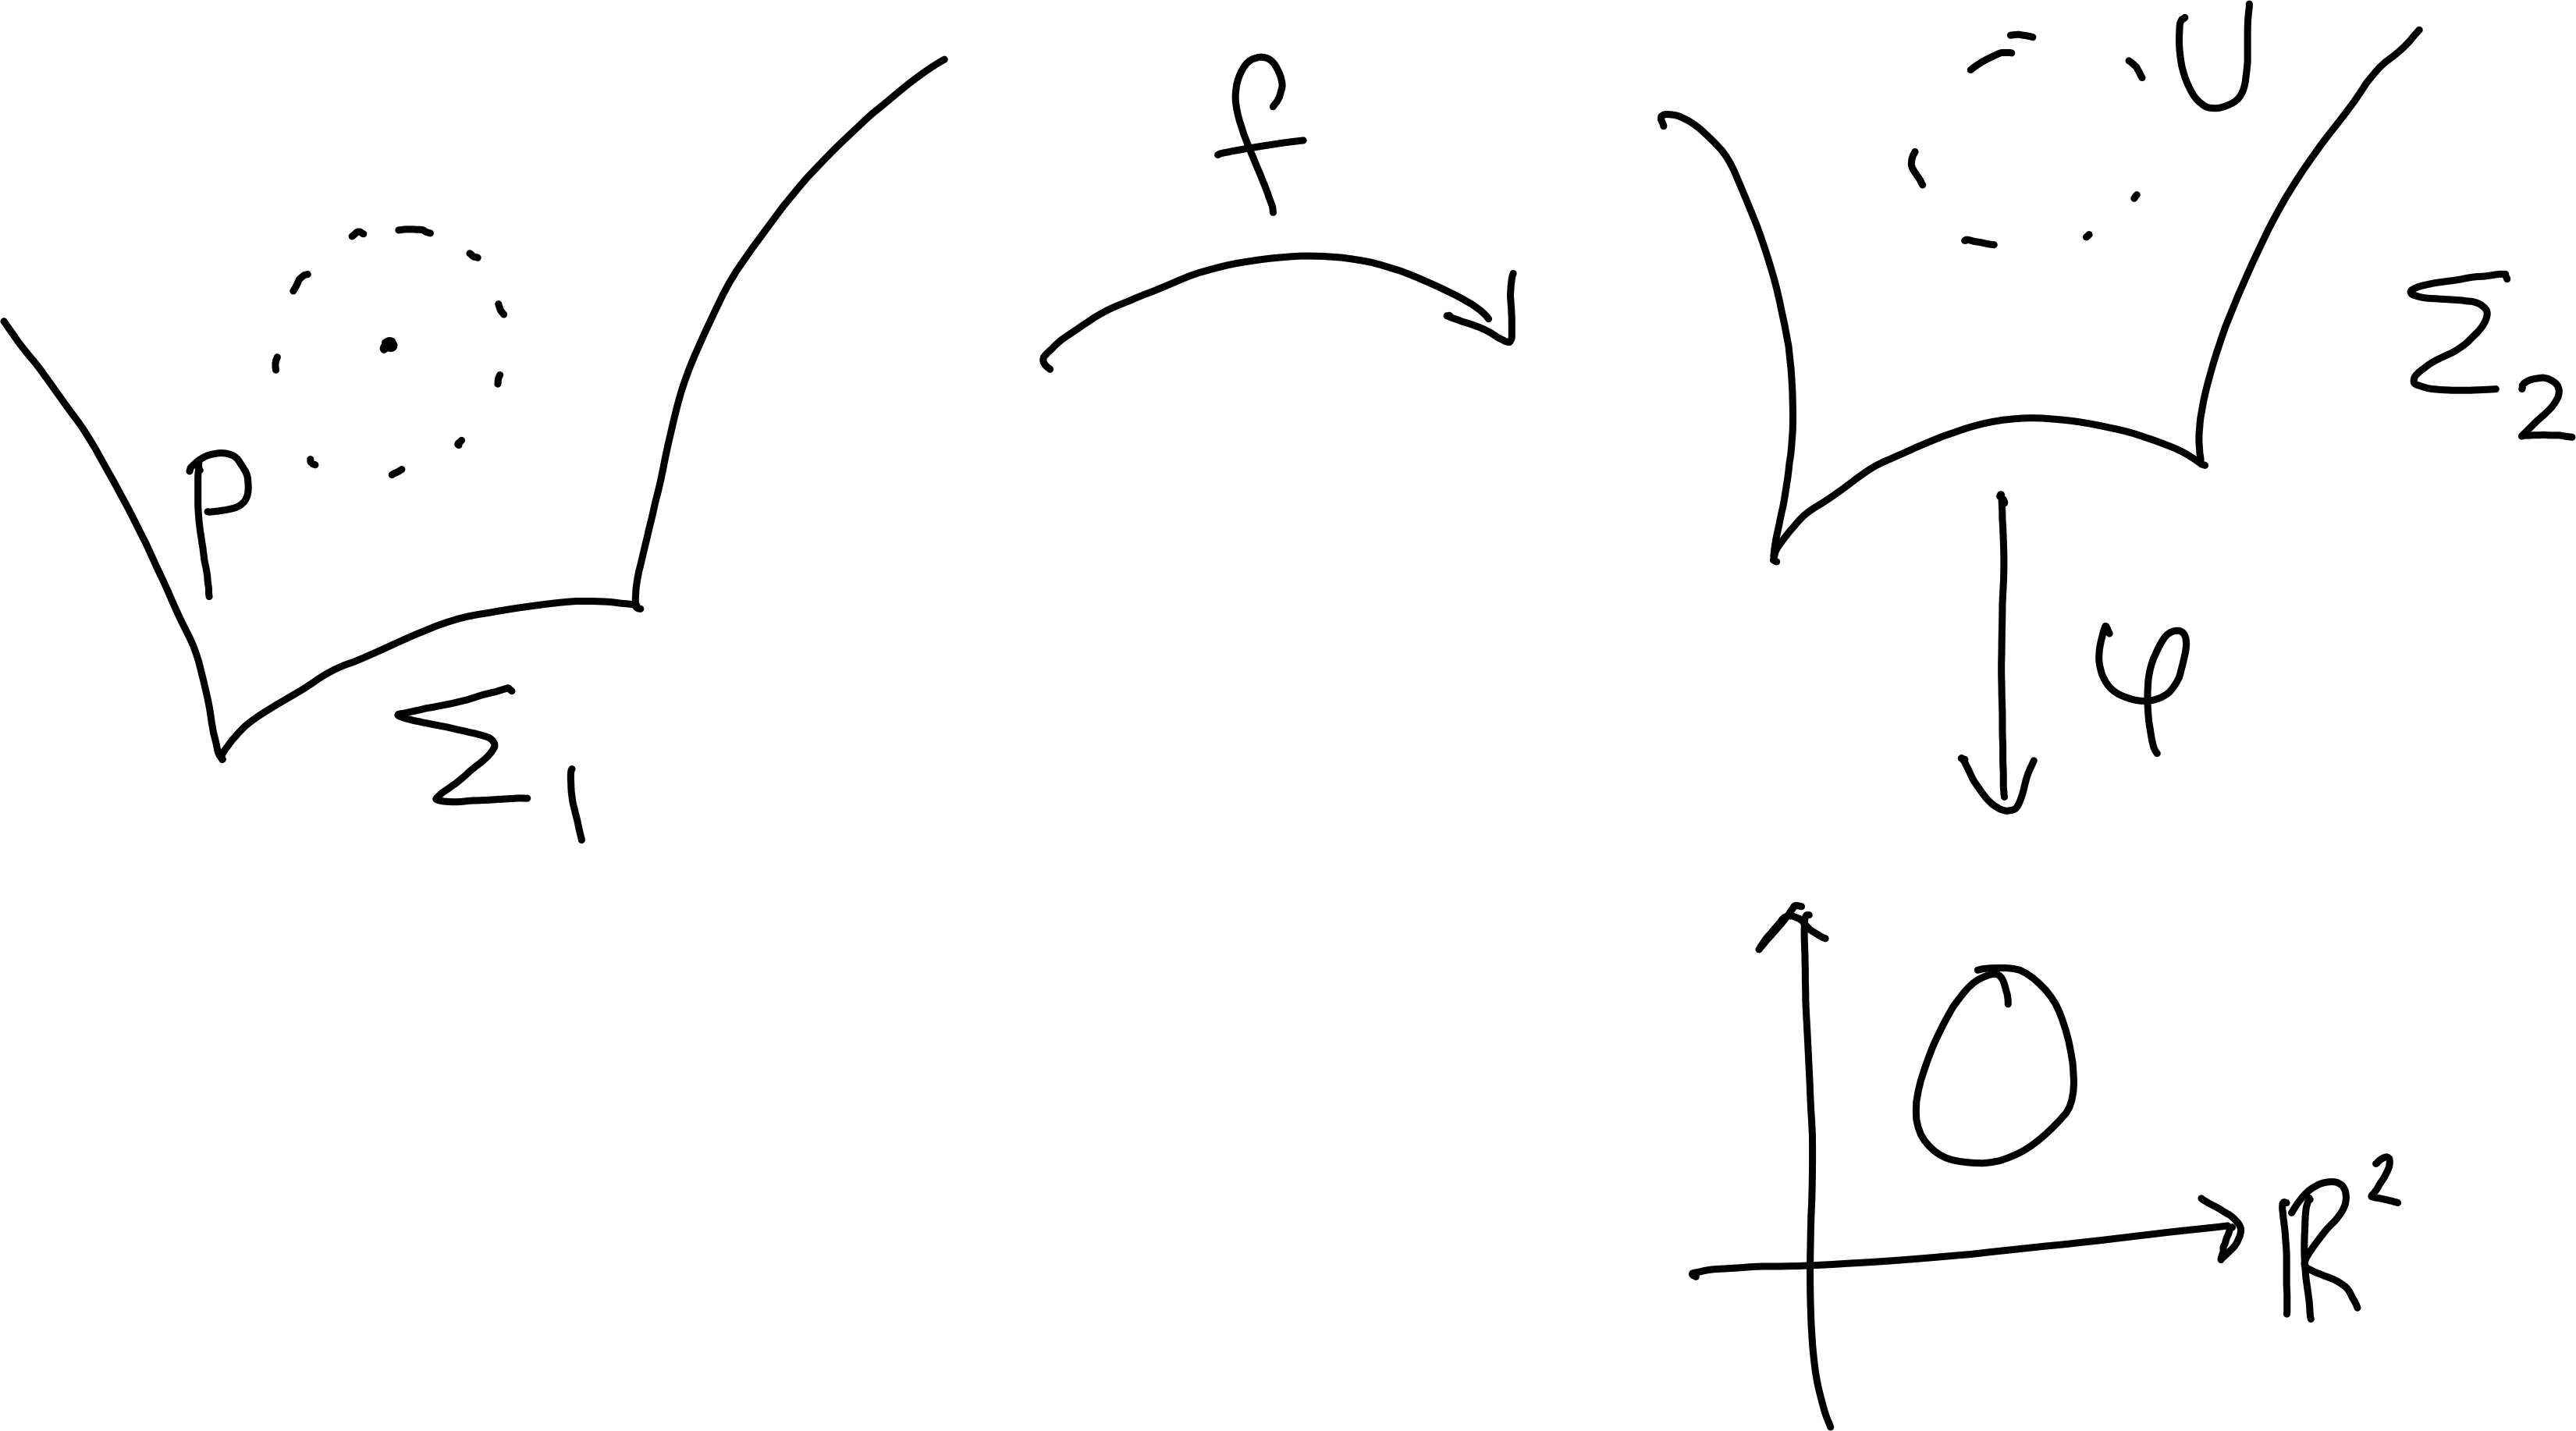
\includegraphics[height=5cm]{03-orientable} 
	\par}

	Consider the atlas on $\Sigma_1$ given by $(f^{-1}(U), \eval{\phi \circ f}_{f^{-1}(U)})$, where $(U, \psi)$ is a chart at $f(p)$ in the oriented atlas for $\Sigma_2$.
	Then, the transition function\footnote{$(\phi_1 \circ f) \circ (\phi_2 \circ f)\inv = \phi_1 \circ \phi_2\inv$} between two such charts is exactly the transition function between charts in the $\Sigma_2$ atlas.
	% In other words, in the maximal smooth atlas that exists a priori for $\Sigma_1$, we will allow charts of the form $(\widetilde U, \widetilde \psi)$ when for all charts $(U, \psi)$ at $f(p)$ in the $\Sigma_2$ atlas, the map $\psi \circ f \circ (\widetilde \psi)^{-1}$ is orientation-preserving.
	% Informally, if the atlas on $\Sigma_2$ was maximal as an oriented atlas, we can recover the previous set of charts.
\end{proof}

\begin{remark}
	\begin{enumerate}
		\item 	There is no sensible classification of the set of all smooth or topological surfaces.
		For instance, $\mathbb R^2 \setminus Z$ for a closed set $Z$ can be shown to yield uncountably many types of homeomorphisms. \\
		However, \underline{compact} smooth surfaces may be classified by their Euler characteristic and their orientability, up to diffeomorphism.
		This theorem will not be proven in this course.
		\item 	There is a definition of orientation-preserving \textit{homeomorphism} that does not rely on the determinant, but that instead relies on some algebraic topology which is not covered in this course.
		The M\"obius band is the surface
		\tikzfig{mobius_band}
		where the dashed lines represent the absence of edges.
		It is provable that an abstract smooth surface is orientable $\iff$ it contains no subsurface (an open set) homeomorphic to the M\"obius band.
		We can therefore say that a topological surface is orientable $\iff$ it contains no subsurface (an open set) homeomorphic to a M\"obius band.
		\item 	We can define other structures on an abstract smooth surface by considering smooth atlases such that if $\varphi_1 \varphi_2^{-1}$ is a transition map, then $D (\varphi_1 \varphi_2^{-1})$ at $x$ belongs to a specific subgroup $G \leq GL(2, \mathbb R)$.
		For example, defining $G = \qty{e}$ leads to Euclidean surfaces.
		The group $GL(1, \mathbb C)$ identified as a subgroup of $GL(2, \mathbb R)$ yields the Riemann surfaces, also $D (\varphi_1 \varphi_2^{-1}) \in GL(1, \mathbb C) \implies \varphi_1 \varphi_2^{-1}$ holomorphic as being in $GL(1, \mathbb C)$ implies that the Cauchy Riemann equations hold.
	\end{enumerate}
\end{remark}

\begin{example}
	For $S^2$ with the atlas of two stereographic projections, we can find the transition map to be
	\begin{align*}
		(u,v) \mapsto \qty(\frac{u}{u^2 + v^2}, \frac{v}{u^2 + v^2})
	\end{align*}
	on $\mathbb R^2 \setminus \qty{0}$.
	This has positive determinant, so $S^2$ is orientable.

	Note we only need to know the determinant at one point in $\mathbb{R}^2 \setminus \qty{0}$ as $\mathbb{R}^2 \setminus \qty{0}$ is a connected set so the determinant of the differential is a super continuous function, so if it has sign positive at one point it must have sign positive on the whole space. If its sign changed it must be $0$ somewhere but we know its a diffeomorphism so the determinant of the differential can't be 0.
\end{example}

\begin{example}
	For the torus $T^2$, we previously found an atlas such that the transition maps are translations of $\mathbb R^2$.
	Hence the torus is an oriented surface, and also a Euclidean surface.
\end{example} 

For surfaces in $\mathbb{R}^3$, we'd like to have orientability dictated by some ``ambient feature'', i.e. we want to be able to just look at the surface and know if its orientable or not.

\subsection{Tangent planes}
Recall that an \textit{affine} subspace of a vector space is a translation of a linear subspace.

\begin{definition}[Tangent Plane]
	Let $\Sigma$ be a smooth surface in $\mathbb R^3$, and $p \in \Sigma$.
	Let $\sigma \colon V \to U \subset \Sigma$ be an allowable parametrisation of $\Sigma$ near $p$, so $V$ is an open subset of $\mathbb R^2$ and $U$ is open in $\Sigma$, such that $\sigma(0) = p$.

	The \vocab{tangent plane} $T_p \Sigma$ of $\Sigma$ at $p$ is the image of $\qty(\eval{D\sigma}_0) \subset \mathbb R^3$, which is a two-dimensional vector subspace of $\mathbb R^3$.
	The \vocab{affine tangent plane} is $p + T_p \Sigma$, which is an affine subspace of $\mathbb R^3$.
\end{definition}

\begin{figure}[h] 
    \centering 
    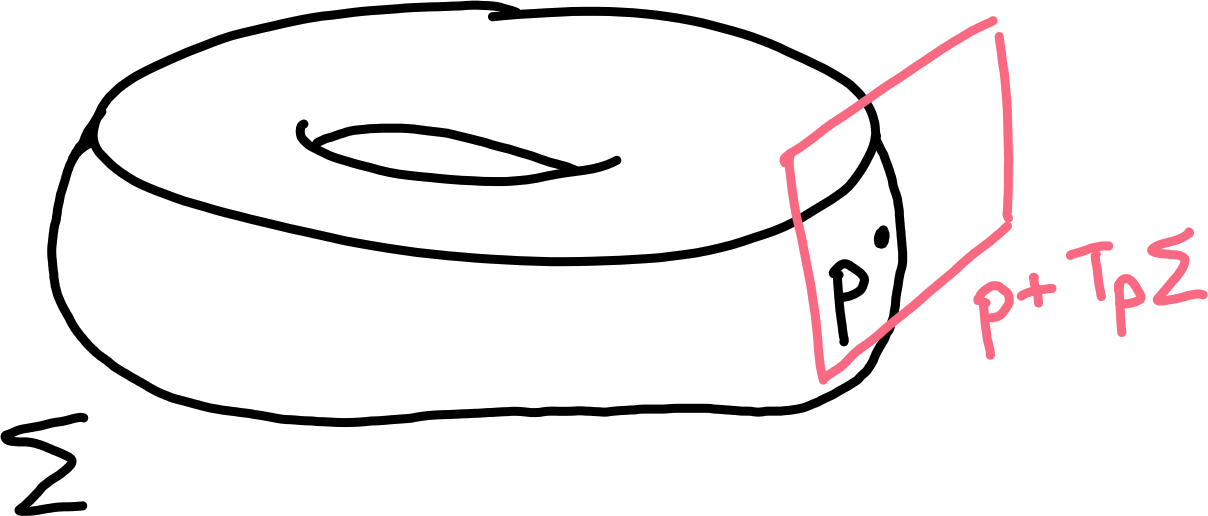
\includegraphics[height=5cm]{03-tangentplane} 
\end{figure}

\begin{remark}
	The affine tangent plane is the `best' linear approximation to a surface $\Sigma$ at a given point.
\end{remark}

\begin{lemma} \label{lem:1.9}
	$T_p \Sigma$ is well-defined, i.e. it's independent of the choice of allowable parametrisation near $p$.
\end{lemma}

\begin{proof}[Proof (i)]
	Suppose $\sigma \colon V \to U$ and $\widetilde \sigma \colon \widetilde V \to \widetilde U$ are allowable parametrisations with $\sigma(0) = \widetilde \sigma(0) = p$.
	There exists a transition map $\sigma^{-1} \circ \widetilde \sigma$, which is a diffeomorphism of open sets in $\mathbb R^2$.
	Therefore,
	\begin{align*}
		\widetilde \sigma = \sigma \circ \underbrace{\qty(\sigma^{-1} \circ \widetilde \sigma)}_{\text{diffeomorphism}}
	\end{align*}
	Hence $\eval{D(\sigma^{-1} \circ \widetilde \sigma)}_{0}$ is an isomorphism.
	Thus, the images of $D \eval{\widetilde \sigma}_0$ and $D \eval{\sigma}_0$ agree.
\end{proof}

\begin{proof}[Proof (ii)]
	Let $\gamma \colon (-\varepsilon, \varepsilon) \to \mathbb R^3$ be a smooth map such that $\gamma$ has image inside $\Sigma$, and $\gamma(0) = p$.
	We will show that $\gamma'(0) \in T_p \Sigma$.
	If $\sigma \colon V \to U$ is an allowable parametrisation with $\sigma(0) = p$ as above, and $\varepsilon$ is sufficiently small such that $\Im \gamma \subset U$, then $\gamma(t) = \sigma(u(t), v(t))$ for some smooth functions $u, v \colon (-\varepsilon, \varepsilon) \to V$.
	Then $\gamma'(t) = \sigma_u u'(t) + \sigma_v v'(t)$ is in the image of $D \eval{\sigma}_t$.
	Thus, $T_p \Sigma = \vecspan \qty{ \gamma'(0) \colon \gamma \text{ as above} }$.
\end{proof}

\begin{definition}[Normal Direction]
	If $\Sigma$ is a smooth surface in $\mathbb R^3$ and $p \in \Sigma$, the \vocab{normal direction} to $\Sigma$ at $p$ is $(T_p \Sigma)^\perp$, the Euclidean orthogonal complement to the tangent plane at $p$.
\end{definition}

\begin{remark}
	For all $p \in \Sigma$, there exist exactly two normalised normal vectors.
\end{remark}

\begin{definition}[Two-Sided]
	A smooth surface in $\mathbb R^3$ is \vocab{two-sided} if it admits a continuous global choice of unit normal vector.
\end{definition}

\begin{lemma} \label{lem:1.10}
	A smooth surface in $\mathbb R^3$ is orientable (as an abstract smooth surface) iff it is two-sided (as a smooth surface in $\mathbb R^3$).
\end{lemma}

\begin{proof}
	Let $\sigma \colon V \to U \subset \Sigma$ be an allowable parametrisation.
	Let $\sigma(0) = p$.
	We will define the positive unit normal with respect to $\sigma$ at $p$ to be the normal vector $n_\sigma(p)$ with the property that $\qty{\sigma_u, \sigma_v, n_\sigma(p)}$ and $\qty{e_1, e_2, e_3}$ are related by a positive determinant change of basis matrix (the two sets of vectors have the same orientation), where $\qty{e_1, e_2, e_3}$ are the standard basis vectors.
	In other words,
	\begin{align*}
		n_\sigma(p) = \frac{\sigma_u \times \sigma_v}{\norm{\sigma_u \times \sigma_v}}
	\end{align*}
	Consider an alternative parametrisation $\widetilde \sigma \colon \widetilde V \to \widetilde U$, where $\widetilde \sigma(0) = p$, such that $\widetilde \sigma$ belongs to the same oriented and smooth atlas as $\sigma$.
	Hence, $\sigma = \widetilde \sigma \circ \varphi$ for some transition map $\varphi = \widetilde \sigma\inv \circ \sigma$.
	Let
	\begin{align*}
		D \eval{\varphi}_0 = \begin{pmatrix}
			\alpha & \beta  \\
			\gamma & \delta
		\end{pmatrix}
	\end{align*}
	Hence,
	\begin{align*}
		\sigma_u = \alpha \widetilde \sigma_u + \gamma \widetilde \sigma_v;\quad \sigma_v = \beta \widetilde \sigma_u + \delta \widetilde \sigma_v
	\end{align*}
	This gives
	\begin{equation}
		\sigma_u \times \sigma_v = \det\qty(D \eval{\varphi}_0) \widetilde \sigma_u \times \widetilde \sigma_v \tag{$\dagger$}
	\end{equation}
	The determinant here is positive since the charts in question belong to an oriented atlas.
	Thus the positive unit normal is intrinsic to the surface, it does not depend on the choice of parametrisation.
	The expression for $n_\sigma(p)$ is continuous since the cross product is continuous, hence $\Sigma$ is two-sided.

	Conversely, if $\Sigma$ is two-sided, there exists a global continuous choice of normal vector, so we can consider the subatlas of the smooth atlas s.t we have a chart $(U,\varphi)$ with $\phi\inv = \sigma$ and $\qty{\sigma_u, \sigma_v, n}$ is an oriented basis of $\mathbb{R}^3$.
	We can make $\qty{\sigma_u, \sigma_v, n}$ have positive orientation by negating $\sigma$.
	By ($\dagger$), the transition maps between such charts are orientation-preserving.
	Hence $\Sigma$ is orientable.
\end{proof}

\begin{remark}
	Given $\gamma : (-\epsilon, \epsilon) \to \mathbb{R}^3$ smooth with $\Im(\gamma) \subset \Sigma$ and $\gamma(0) = p$.
	$\gamma(t) = \sigma(u(t), v(t))$ so $\gamma'(0) = \eval{D \sigma}_0(u'(0), v'(0)) \in T_p \Sigma$.
	This gives that $T_p \Sigma = \vecspan \qty{ \gamma'(0) \colon \gamma \text{ as above} } =$ ``tangent vectors to curves in $\Sigma$''.
\end{remark} 

\begin{lemma}
	If $\Sigma$ is a smooth surface in $\mathbb R^3$ and $A \colon \mathbb R^3 \to \mathbb R^3$ is a smooth map which preserves $\Sigma$ setwise, then $\eval{DA}_p \in L(\mathbb R^3, \mathbb R^3)$ maps $T_p \Sigma$ to $T_{A(p)} \Sigma$ for $p \in \Sigma$.
\end{lemma}

\begin{proof}
	Let $\gamma \colon (-\varepsilon, \varepsilon) \to \mathbb R^3$ be a smooth map such that its image lies on $\Sigma$, and $\gamma(0) = p$.
	Recall that $T_p \Sigma$ is spanned by $\gamma'(0)$ for such curves $\gamma$.
	Now, consider $A \circ \gamma \colon (-\varepsilon, \varepsilon) \to \mathbb R^3$, which also has image $\Sigma$, and
	\begin{align*}
		D \eval{A}_{\gamma(0)} \circ D \eval{\gamma}_0 = D \eval{A}_p \qty(\gamma'(0)) = D \eval{(A \circ \gamma)}_0 \in T_{A(p)} \Sigma
	\end{align*}
\end{proof}

\begin{example}[Unit Sphere]
	Let $S^2 \subset \mathbb{R}^3$ be the unit sphere.
	The normal vector at $p$ is the line through the origin and $p$; indeed, since $SO_3$ acts transitively on $S^2$, it suffices to check at one point, such as the north pole.
	We can choose the outward-facing normal vector to be the positive normal, denoted $n(p)$.
	$S^2$ is two-sided by the construction of this normal vector, hence $S^2$ is orientable.

	Alternatively, take any $\gamma : (-\epsilon, \epsilon) \to S^2$ with $\gamma(0) = p$.
	$\norm{\gamma(t)}^2 = 1$, so differentiating at $t = 0$, $2 \inner{\gamma'(0), p} = 0$ so $(T_p S^2)^\perp = \mathbb{R} p = \{xp: x \in \mathbb{R}\}$.
	Let $n(p) = p$, clearly a global continuous choice of normal vector so $S^2$ is 2-sided.
\end{example}

\begin{example}[M\"obius Band]
	Walk around the unit circle in the $xy$-plane and take an open interval of length 1.
	Rotate this line in the $cz$-plane as we move around the circle, s.t. it has rotated by $\frac{\theta}{2}$ after moving an angle $\theta$ in the circle (see picture).
	After a full turn the segment returns to its original position but with end points inverted. \\
	One embedding of the M\"obius band in $\mathbb R^3$ is
	\begin{align*}
		\sigma(t,\theta) = \qty(\qty(1 - t \sin \frac{\theta}{2})\cos \theta, \qty(1 - t \sin \frac{\theta}{2})\sin \theta, t \cos \frac{\theta}{2})
	\end{align*}
	where $(t,\theta) \in V_1 = \qty{t \in \qty(-\frac{1}{2}, \frac{1}{2}), \theta \in (0,2\pi)}$ or \\$(t,\theta) \in V_2 = \qty{t \in \qty(-\frac{1}{2}, \frac{1}{2}), \theta \in (-\pi, \pi)}$. \\
	This gives us the standard M\"obius band parametrically, I don't think its worthwhile trying to understand why exactly it works or what the explanation even means.

	We can check that if $\sigma_i$ is $\sigma$ on $V_i$, then $\sigma_i$ is allowable.
	Further,
	\begin{align*}
		\sigma_t \times \sigma_\theta = \qty(-\cos\theta \cos\frac{\theta}{2}, -\sin\theta \cos\frac{\theta}{2}, -\sin\frac{\theta}{2}) \equiv n_\theta
	\end{align*}
	which is already normalised.
	As $\theta \to 0$ from above, $n_\theta \to (-1,0,0)$.
	As $\theta \to 2\pi$ from below, $n_\theta \to (1,0,0)$.
	Hence, the surface is not two-sided.
\end{example}
